\subsection{Mallob Integration}
- how we integrated CrowdHTN with Mallob
- this is done by implementing a job interface in Mallob
- the interface code can be found online in the Mallob repository \footnote{https://github.com/domschrei/mallob}
- and additionally a function to read an instance
- give a short overview of the interface
- a job is internally implemented as a state machine
- the state diagram is found at \ref{figure: mallob state diagram}
- from \cite{schreiber2021scalable} we know that Mallob aims to deliver latencies in the millisecond range
- messages may only ever be sent from the main thread

\begin{algorithm}
	\caption{The Mallob job interface}
	\label{algo - mallob interface}
	void appl\_start()\;
	void appl\_suspend()\;
	void appl\_resume()\;
	void appl\_terminate()\;
	void appl\_solved()\;
	JobResult appl\_getResult()\;
	void appl\_communicate()\;
	void appl\_communicate(source, mpi\_tag, message)\;
	void appl\_memoryPanic()\;
\end{algorithm}

\subsubsection{Added Fault Tolerance}
As a scheduler, within a single execution Mallob may work on any number of jobs making it necessary that jobs do not crash. This imposes additional challenges for TOHTN planning, as we have seen in section \ref{prelim: tohtn complexity} that TOHTN planning is EXPSPACE hard, meaning we may often run out of memory and will be subsequently shut down by the operating system. Luckily, the Mallob job interface we see in algorithm \ref{algo - mallob interface} does provide a function for this case. Mallob does periodically check available memory and if it threatens to run out triggers the \textit{appl\_memoryPanic()} function. In our case we have implemented it as clearing out both our local fringe of search nodes and the loop detection information, resetting the local search. Afterwards, an affected PE will simply resume the work stealing and message other PEs to re-join the work at reduced memory footprint. While this does means we loose parts of the search space, the alternative would be to immediately return without a plan. Additionally, with the restarting mechanism we introduced in section \ref{ld - completeness} CrowdHTN retains completeness even in this case.

\subsubsection{Achieving millisecond latencies}
- big operations are put into separate threads
- this includes the \textit{start} function where the instance gets parsed and the CrowdHTN worker is initialized
- similarly, the CrowdHTN worker is put into a separate thread which is started in \textit{start}
- the functions \textit{suspend}, \textit{terminate} communicate with the CrowdHTN worker via atomics
- \textit{resume} is realized via a condition variable to wake up the worker thread
- where needed, locking is kept to an absolute minimum: messages are communicated from and to the CrowdHTN worker via dynamic arrays (realized through \textit{std::vector}) which are locked only for swapping the metadata in and out

\subsubsection{Handling version increases}
- false positives in loop detection necessitate restarts \ref{improv: loop detection}
- as a result, we need to invalidate all workers and start anew
- broadcast new versions as they happen to enforce fast updates
- loop detector size:

\begin{figure}
	\caption{State transition diagram of a Mallob job}
	\label{figure: mallob state diagram}
	\centering
	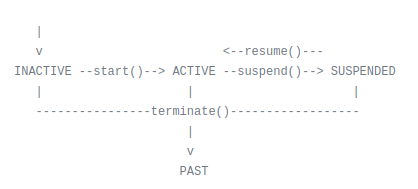
\includegraphics{images/prelim/mallob_state_diagram}
\end{figure}

\subsection{Global Loop Detection}
In section \ref{ld - global} we introduced a distributed loop detection mechanism based on regularly shared bloom filters. This leaves us with two problems, first performing the associated allreduction while the PEs assigned to the job may change at any time and secondly performing the restarts which are required if the bloom filter fills up. \\
In both cases we will make use of the specific way in which Mallob organizes the PEs assigned to a job which we have already explained in section \ref{prelim: mallob}. The two properties we rely on are the fact that PEs are internally structured as a binary tree with parent and child information available to us and the fact that the root PE will remain assigned to a job during the job's full duration.

\paragraph{Performing the Reduction}
The all-reduction of our loop detection data is initiated by the root PE and performed in three phases. 
\begin{itemize}
	\item Initiating the reduction
	\item Aggregating information upwards
	\item Broadcasting the aggregated information
\end{itemize}
The root PE is responsible for initializing the all-reduction. It does so by starting a broadcast, sending an initialization message to all it's children. Upon receiving a reduction initialization message, a PE both forwards the message to its own children and prepares the local loop detection data. 

- init: allows for a centralized start

- multiple phases:
	- 
- root induces a new sharing operation, broadcasting this information

- receiving PEs initiate their local operation, get local data, forward broadcast
- from the leaves we propagate the information upwards
- if the initiation broadcast is returned or a worker is suspended after receiving it, it's parent pretends that a message containing no data was sent
- this whole operation takes logarithmic time in the number of PEs
- if we enforce 'response exists' from bottom to top we will always conclude the operation even when PEs change

\subsubsection{Loop Detection Induced Restarts}
In section \ref{ld - global} we introduced a global loop detection mechanism based on regularly shared bloom filters. One of the problems this induces is that we need to induce restarts to increase the size of the bloom filter in order to avoid increasing false positive rates. The main problem here is that for different PEs the global bloom filter will fill up at different times. This is due to the fact that different PEs may be assigned to our job for different spans in time which may be further disjointed as PEs are suspended and subsequently reassigned to a job. However, to uphold our guarantees we want to restart all our PEs as soon as a single PE needs to do so.\\
We solve this problem by relying on the way in which Mallob organizes the PEs assigned to a single job. In section \ref{prelim: mallob} we described this organization into a binary tree of PEs. The crucial property here is that the root PE is guaranteed to stay assigned to the same job during the jobs full duration. It follows that the root PE is present during every sharing of loop detection information and that, if any PEs global bloom filter is full this implies that the root PEs global bloom filter is also full. \\
This fact allows us to only ever check on the root PE whether the global bloom filter is full and institute a restart if needed. Doing so lets us avoid any problems that would stem from all PEs performing such checks, such as multiple PEs instituting restarts at the same time.
